\documentclass{standalone}
\usepackage{tikz}
\begin{document}
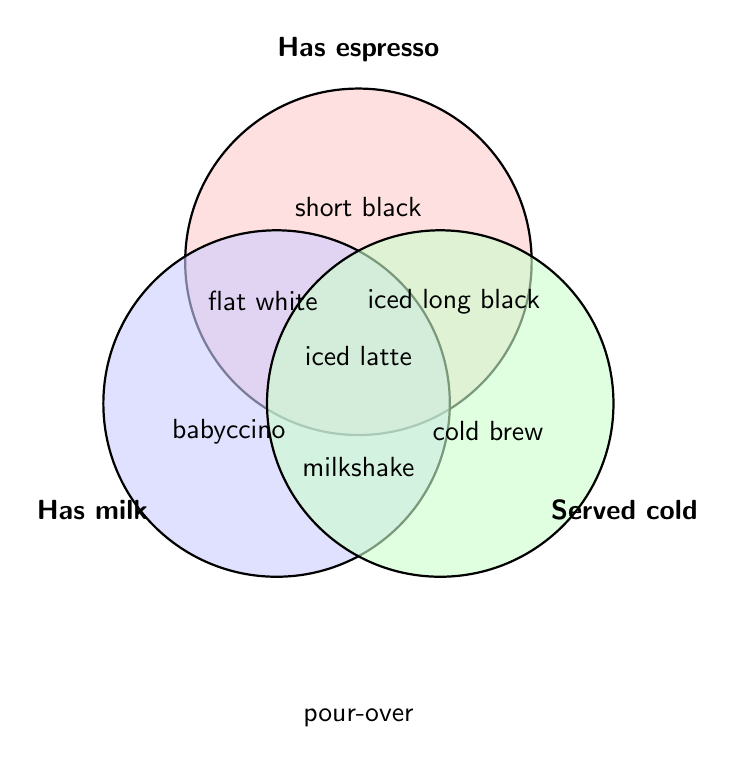
\begin{tikzpicture}[font=\sffamily]
  % Circles
  \draw[thick, fill=red!20, fill opacity=0.6] (90:1.2) circle (2.2);
  \draw[thick, fill=blue!20, fill opacity=0.6] (210:1.2) circle (2.2);
  \draw[thick, fill=green!20, fill opacity=0.6] (330:1.2) circle (2.2);

  % Labels
  \node[font=\sffamily\bfseries] at (90:3.9) {Has espresso};
  \node[font=\sffamily\bfseries] at (210:3.9) {Has milk};
  \node[font=\sffamily\bfseries] at (330:3.9) {Served cold};

  % Drinks in regions
  \node at (90:1.9) {short black};                 % espresso only
  \node at (210:1.9) {babyccino};                  % milk only
  \node at (330:1.9) {cold brew};                  % cold only
  \node at (150:1.4) {flat white};                 % espresso + milk
  \node at (30:1.4) {iced long black};             % espresso + cold
  \node at (270:1.4) {milkshake};                  % milk + cold
  \node at (0,0) {iced latte};                     % all three
  \node at (0,-4.6) {pour-over};                   % outside all
\end{tikzpicture}
\end{document}
